\section{Conjuntos de datos}\label{sec:datos}
En este capítulo describimos los conjuntos de datos (datasets) utilizados en nuestros experimentos, tanto para la tarea de clasificación de niveles como para la de adaptación lingüística. Presentamos primero los criterios de selección y la tipología de los textos considerados (\Cref{subsection:tipos_textos}), seguidos de una descripción detallada de los corpus existentes y la conformación de nuestro dataset combinado (Custom Dataset) (\Cref{subsection:datasets}). Luego presentamos el corpus que armaron los organizadores de la tarea de simplificación de TSAR (\Cref{subsection:dataset_tsar}). Finalmente, detallamos el proceso de construcción y validación de un nuevo recurso de adaptaciones alineadas al CEFR, desarrollado específicamente para suplir las necesidades actuales de recursos específicos (\Cref{subsection:dataset_adaptacion}).

\subsection{Tipos de textos y criterios de selección}\label{subsection:tipos_textos}
Antes de detallar los corpus utilizados, es preciso definir las dimensiones que caracterizan a los textos en el ámbito del procesamiento de lenguaje natural (NLP) para L2. La elección de los datos está condicionada por tres ejes fundamentales: la granularidad, el origen de la autoría y el género textual.

\subsubsection*{Granularidad y coherencia}
En tareas de clasificación y adaptación, los textos pueden abordarse desde distintos niveles de granularidad: oraciones, párrafos o documentos completos. Para este trabajo, se optó por utilizar textos completos (documentos), basándonos en las siguientes premisas:
\begin{itemize}
    \item \textbf {Autocontención:} Los documentos completos preservan la estructura lógica y el contexto necesario para que el contenido sea plenamente comprensible sin dependencias externas.
    \item \textbf {Fiabilidad de la etiqueta:} La clasificación de un texto suele estar determinada por su pasaje más complejo. Si un texto de nivel C1 se subdivide, no existe garantía de que cada uno de sus párrafos u oraciones conserve dicha complejidad; por el contrario, es probable que muchas de sus partes, aisladas, presenten características de niveles inferiores (como A2 o B1). Etiquetar automáticamente fragmentos basándose en el nivel del documento original introduciría un ``ruido'' significativo en el dataset.

    \item \textbf {Complejidad discursiva:} La dificultad de un nivel superior (como C1 o C2) no reside solo en el vocabulario o la sintaxis de oraciones aisladas, sino en la relación cohesiva entre párrafos y el manejo de la retórica, elementos que se pierden al fragmentar la unidad textual.
\end{itemize}

\subsubsection*{Autoría y competencia lingüística}
Los materiales pueden dividirse según la competencia de quien los genera: textos producidos por aprendices (learner corpora) o textos creados por expertos (docentes, lingüistas o hablantes nativos). En esta investigación, se decidió trabajar exclusivamente con textos creados por expertos debido a que:

\begin{itemize}
    \item \textbf {Modelado de la norma:} Para tareas de adaptación y generación, los textos de expertos sirven como un estándar de corrección gramatical y pragmática que el modelo debe emular.
    \item \textbf {Precisión pedagógica:} Los textos diseñados por expertos para exámenes o libros de texto están calibrados específicamente para representar los descriptores del CEFR, evitando los errores interlingüísticos comunes en los aprendices que podrían confundir al modelo durante el entrenamiento.
\end{itemize}

\subsubsection*{Género y diversidad textual}
En cuanto a la tipología, los textos abarcan una amplia gama de géneros, incluyendo documentos oficiales, artículos periodísticos, contenido web y transcripciones de conversaciones. No se impuso una restricción estricta sobre el tipo de texto, ya que el objetivo es que el sistema sea capaz de operar en escenarios reales y diversos, reflejando la heterogeneidad de materiales a los que un estudiante de L2 se enfrenta habitualmente.


\subsection{Datasets de textos clasificados con nivel CEFR}\label{subsection:datasets}
En el campo de NLP aplicado a L2 learners, se han desarrollado recientemente varios datasets de textos en inglés clasificados por nivel CEFR. En este trabajo utilizamos principalmente dos de ellos:
\begin{itemize}
    \item CEFR Levelled English Texts (CLET) \parencite{kagle}.
    \item Cambridge English Readability Dataset (CERD) \parencite{Imperial2025}.
\end{itemize}

La diferencia fundamental entre ambos radica en la forma en que los textos fueron etiquetados. En CLET, la mayor parte de las etiquetas fueron asignadas automáticamente utilizando la herramienta Text Inspector. En cambio, en CERD, las etiquetas fueron asignadas por expertos humanos, lo que otorga una mayor fiabilidad a las clasificaciones.

Otra diferencia importante es que CERD cubre únicamente los niveles A2 a C2, mientras que CLET incluye ejemplos de nivel A1, lo que resulta clave para tener cobertura completa de la escala CEFR.

\subsubsection*{CEFR Levelled English Texts (CLET)}

El dataset CLET consiste en 1,494 textos clasificados automáticamente. Se puede observar la distribución por nivel CEFR en la \Cref{tab:kaggle}.
\begin{table}[H]
\centering
\begin{tabular}{@{}cllllll@{}}
\toprule
\textbf{Nivel CEFR}         & A1  & A2  & B1  & B2  & C1  & C2  \\ \midrule
\textbf{Cantidad de textos} & 288 & 272 & 205 & 286 & 241 & 202 \\ \bottomrule
\end{tabular}
\caption{Distribución de la clasificación de textos para Kaggle.}
\label{tab:kaggle}
\end{table}

Los textos provienen de fuentes variadas como The British Council, ESLFast y el CNN/DailyMail dataset. El corpus incluye diferentes tipos textuales: diálogos, descripciones, historias cortas y noticias.

Durante las primeras etapas de nuestro trabajo utilizamos este dataset como base. Sin embargo, tras una revisión realizada junto con profesores de inglés como lengua extranjera, detectamos que una proporción considerable de textos se encontraba mal clasificada. Esto motivó la búsqueda de un dataset de mayor calidad.

\subsubsection*{Cambridge English Readability Dataset (CERD)}
El dataset CERD contiene 331 textos extraídos de pasajes de lectura de los cinco exámenes principales de Cambridge English KET (A2), PET (B1), FCE (B2), CAE (C1), CPE (C2). Su distribución por nivel se puede observar en la \Cref{tab:CERD}.

\begin{table}[H]
\centering
\resizebox{\textwidth}{!}{%
\begin{tabular}{@{}cccccc@{}}
\toprule
\textbf{Nivel CEFR}         & KET (A2) & PET (B1) & FCE (B2) & CAE (C1) & CPE (C2) \\ \midrule
\textbf{Cantidad de textos} & 64       & 60       & 71       & 67       & 69       \\ \bottomrule
\end{tabular}%
}
\caption{Distribución de la clasificación de textos para CERD.}
\label{tab:CERD}
\end{table}

La principal ventaja de CERD es la calidad de la anotación: al estar directamente vinculada a los exámenes oficiales de Cambridge, cada texto tiene un nivel de dificultad CEFR claramente definido y validado por expertos.

\subsubsection*{Custom Dataset}
Para adaptar estos datasets a la tarea que estamos realizando, la cual tiene todos los niveles CEFR, y dado que CERD no contiene textos de nivel A1, construimos un dataset combinado, al que denominamos CUSTOM dataset. A este dataset se le agregan 65 textos de nivel A1 seleccionados manualmente de CLET por profesores de inglés como segunda lengua.

Para llevar adelante nuestros experimentos, realizamos un particionado estratificado del dataset Custom en tres subconjuntos. La estratificación asegura que la proporción de niveles CEFR se mantenga similar en cada división. La distribución final de cada partición se puede observar en la \Cref{tab:Custom}.

\begin{table}[H]
\centering
\begin{tabular}{@{}cccccccc@{}}
\toprule
\textbf{Partición} & \textbf{Total de textos} & \textbf{A1} & \textbf{A2} & \textbf{B1} & \textbf{B2} & \textbf{C1} & \textbf{C2} \\ \midrule
Train          & 316 & 52 & 51 & 48 & 57 & 53 & 55 \\
Eval           & 39  & 6  & 6  & 6  & 7  & 7  & 7  \\
Holdout        & 41  & 7  & 7  & 6  & 7  & 7  & 7  \\ \bottomrule
\end{tabular}%
\caption{Distribución de la clasificación de textos para las particiones del dataset Custom.}
\label{tab:Custom}
\end{table}

El rol de cada partición es el siguiente:
\begin{itemize}
    \item Train: entrenamiento y fine-tuning de los LLMs.
    \item Eval: evaluación intermedia durante la experimentación, sin que los modelos hayan sido entrenados con estos textos.
    \item Holdout: evaluación final, estrictamente reservada para medir el rendimiento real en textos no vistos.
\end{itemize}

Además de la distribución por nivel CEFR, se analizó la distribución de la longitud de los textos en cada partición. La \Cref{fig:densidad_tokens_cefr} muestra la densidad de tokens por nivel CEFR para el dataset Custom, evidenciando que los textos de niveles superiores (C1 y C2) tienden a ser más extensos que los de niveles inferiores (A1 y A2), lo cual es consistente con las expectativas pedagógicas y lingüísticas asociadas a cada nivel de competencia.

\begin{figure}[H]
  \centering
  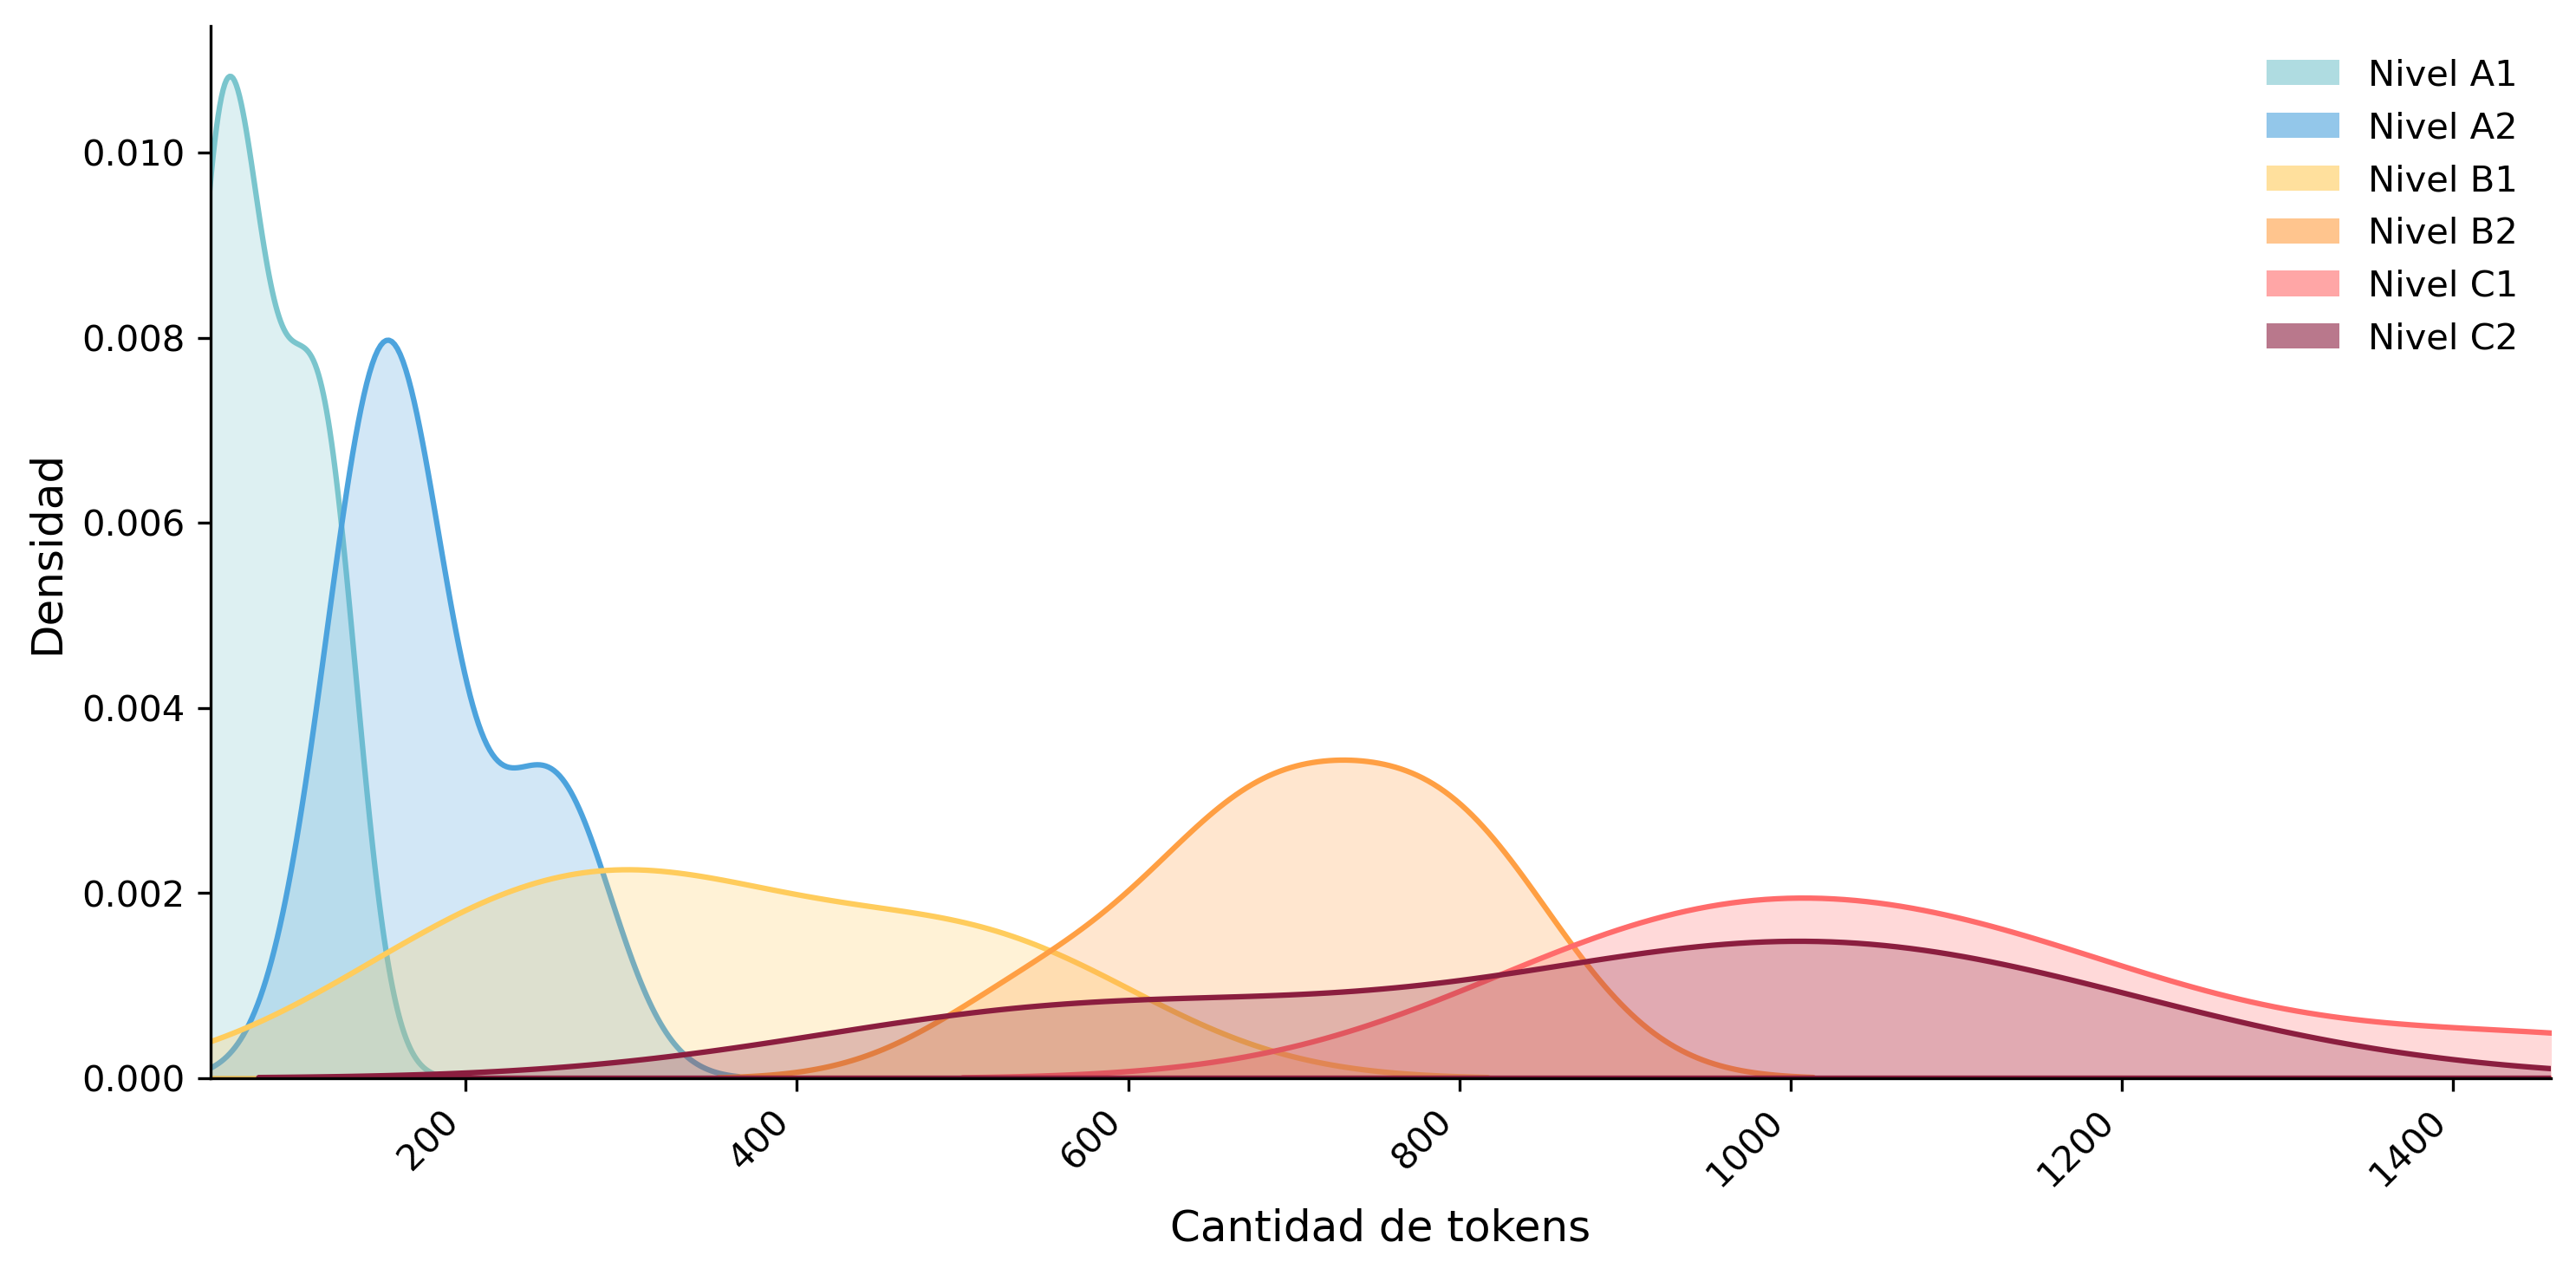
\includegraphics[width=\textwidth]{Graficos_Tesis/densidad_tokens_cefr_superpuesta.png}
  \caption{Densidad de palabras por nivel, medidos en tokens para el dataset Custom.}
  \label{fig:densidad_tokens_cefr}
\end{figure}

\subsection{Corpus de la Shared Task TSAR 2025}\label{subsection:dataset_tsar}
El dataset principal utilizado para los experimentos de adaptación fue diseñado específicamente para la shared task TSAR 2025 \parencite{alva-manchego-etal-2025-findings}, con el objetivo de dar soporte a la simplificación controlada por niveles de legibilidad alineados con el marco CEFR.

\subsubsection*{Fuente de los Datos}
Los textos originales fueron extraídos de la plataforma LearnEnglish del British Council, un recurso de acceso abierto que ofrece contenido pedagógico curado para estudiantes de inglés. El material seleccionado consiste en pasajes de lectura graduados, escritos y revisados por educadores profesionales.

Para la tarea de simplificación, se seleccionó un subconjunto de textos etiquetados originalmente como C1 (Avanzado) y B2 (Intermedio-alto). Estos niveles fueron elegidos debido a que poseen una complejidad léxica y sintáctica suficiente para permitir una transformación significativa hacia niveles inferiores.

\subsubsection*{Proceso de Anotación y Calidad}
El proceso de anotación consistió en generar versiones simplificadas de los textos fuente (C1 y B2) hacia los niveles objetivo B1 (Intermedio) y A2 (Básico-alto). Esto resultó en dos versiones simplificadas por cada texto original. El dataset se distribuyó en dos particiones:
\begin{itemize}
\item \textbf{Trial data:} 20 instancias simplificadas por un único anotador, utilizadas para el desarrollo de los sistemas.
\item \textbf{Test data:} 80 instancias simplificadas por dos anotadores, reservadas para la evaluación oficial de la competencia.
\end{itemize}

Todos los anotadores fueron profesores de inglés como lengua extranjera (EFL) familiarizados con el marco CEFR. Antes de la fase principal, completaron una tarea de calificación para asegurar la consistencia en los criterios de simplificación. Las guías de anotación exigían preservar el significado original, reducir la complejidad lingüística de acuerdo con el nivel objetivo y mantener la gramaticalidad y fluidez del texto resultante.

\subsubsection*{Validación del Dataset}
Dada la naturaleza del trabajo de los expertos (quienes trabajaron sobre subconjuntos disjuntos), la fiabilidad del dataset no se midió mediante acuerdo inter-anotador, sino comparando los niveles asignados manualmente con las predicciones de un modelo evaluador automático de CEFR. El error cuadrático medio (RMSE) promedio fue de 0.6, lo que indica un alineamiento moderado y aceptable considerando la subjetividad inherente a los juicios humanos sobre los niveles de competencia lingüística.

\subsubsection*{Limitaciones del Recurso}
Es importante señalar que el dataset presenta un formato a nivel de párrafo. Si bien existen otros recursos a nivel de oración, la elección de párrafos en TSAR 2025 responde a la necesidad de evaluar la coherencia discursiva en la adaptación, un aspecto central para materiales pedagógicos reales. Asimismo, aunque el dataset se limita al dominio de inglés del British Council, representa un nuevo estándar de oro (gold-standard) paralelo para la comunidad de investigación en simplificación controlada por niveles de suficiencia.

\subsection{Dataset de adaptaciones}\label{subsection:dataset_adaptacion}
Una de las principales limitaciones en el área es la ausencia de datasets que contengan pares de textos donde uno es la adaptación del otro a otro nivel CEFR. Si bien existen corpus de simplificación (como Simple English Wikipedia \parencite{wikipedia}), estos no están organizados de acuerdo con la escala CEFR ni orientados a contextos de enseñanza de segundas lenguas.

Para suplir esta carencia, planteamos un dataset propio de adaptaciones, creado en colaboración con profesores de inglés como segunda lengua con amplia experiencia, donde cada ejemplo consiste en un par de textos donde uno es la adaptación del otro hacia un nivel CEFR distinto (ya sea hacia mayor o menor complejidad).

Este dataset se está construyendo actualmente y constituye un recurso inédito en el dominio y representa un aporte significativo. Su diseño permite evaluar experimentalmente la capacidad de los LLMs no solo para clasificar textos por nivel CEFR, sino también para generar adaptaciones pedagógicamente adecuadas a perfiles concretos de estudiantes L2.

El proceso de construcción de este recurso sigue un protocolo de refinamiento iterativo en tres etapas, combinando la capacidad generativa de los modelos de lenguaje de gran escala (LLMs) con el criterio pedagógico de expertos humanos:

\begin{itemize}
    \item \textbf{Generación Sintética Inicial:} Se utilizara el modelo Llama 3.1 8B para realizar la adaptación de los textos base hacia los niveles objetivo del CEFR. Se diseñaron prompts específicos para que el modelo ajustara la complejidad léxica y sintáctica manteniendo la coherencia semántica del texto original.

    \item \textbf{Revisión y Corrección por Expertos:} Los textos generados seran sometidos a un proceso de edición por parte de profesores de inglés (L2) con amplia experiencia. En esta fase, los expertos no solo corregiran imprecisiones lingüísticas, sino que ajustaran el contenido para asegurar una alineación real con los descriptores del CEFR. Un subproducto valioso de esta etapa sera la recolección de observaciones cualitativas sobre las adaptaciones originales, lo que permitira identificar debilidades sistemáticas del modelo Llama 3.1 8B, tales como cambiar nombres o adjetivos (ej: ``violet'' por ``red'') o la inclusión de conocimiento del LLM que no estaba originalmente (ej: descripción de qué es un meteorito).

    \item \textbf{Validación Cruzada:} Finalmente, los textos revisados seran validados por un segundo grupo de profesores para asegurar el acuerdo inter-evaluador. Este paso garantiza que el nivel CEFR asignado sea consistente y no dependa del criterio subjetivo de un único experto.
\end{itemize}